\subsection{\large{\textit{tP}4-PdO (Direct)}}\vspace{-0.1in}
Palladium Oxide


\begin{figure}[H]
\begin{minipage}{0.34\textwidth}\centering
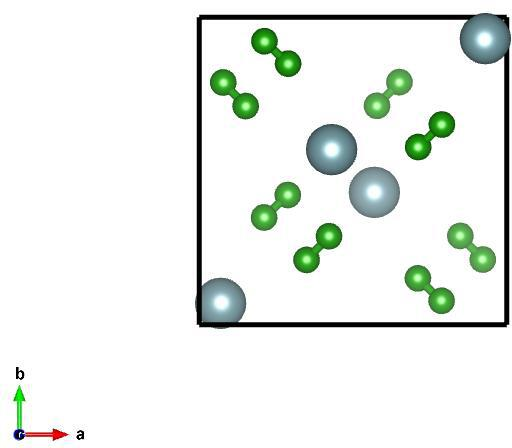
\includegraphics[width=0.9\linewidth,height=2in,keepaspectratio]{/Users/rosecers/work_folders/structures_for_photonics/reference/ref_inp/workspace/3ffeff60e1ef4fe0842f6f61826d67b2/final_images/analog_trim.jpg}\\
\small{Image of \textit{tP}4-PdO, generated by Vesta}
\end{minipage}\hfill
\begin{minipage}{0.65\textwidth}\raggedright
{\setlength{\mathindent}{0cm}
\begin{equation*}
\begin{split}&\boldsymbol{a_1} = \ \hat{x}\\[-8pt]
&\boldsymbol{a_2} = \ \hat{y}\\[-8pt]
&\boldsymbol{a_3} = 1.759075899\ \hat{z}
\end{split}
\end{equation*}}

\textbf{Space Group:}	131\hspace{0.5in}\textbf{Point Group:}	$4/mmm$\\
\textbf{Crystallographic Open Database} \#1009031\\
\textbf{Structure DOI: }\url{10.1107/S0365110X53001800}

\end{minipage}\hfill
\end{figure}
\vspace{-0.25in}


\begin{figure}[H]
\begin{minipage}{0.9\textwidth}\centering
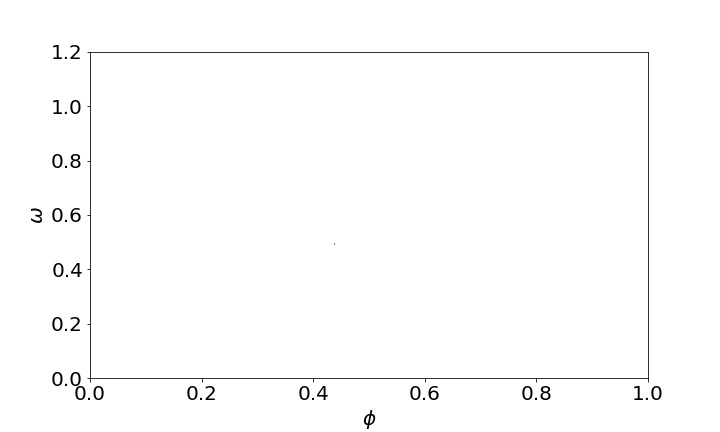
\includegraphics[width=0.9\linewidth,height=2.5in,keepaspectratio]{/Users/rosecers/work_folders/structures_for_photonics/reference/ref_inp/workspace/3ffeff60e1ef4fe0842f6f61826d67b2/final_images/gap_atlas.jpg}
\\
\end{minipage}\hfill\caption{Gap Atlas across filling fraction $\phi$ and frequency $\omega$}
\end{figure}


\begin{figure}[H]
\begin{minipage}{0.5\textwidth}\centering
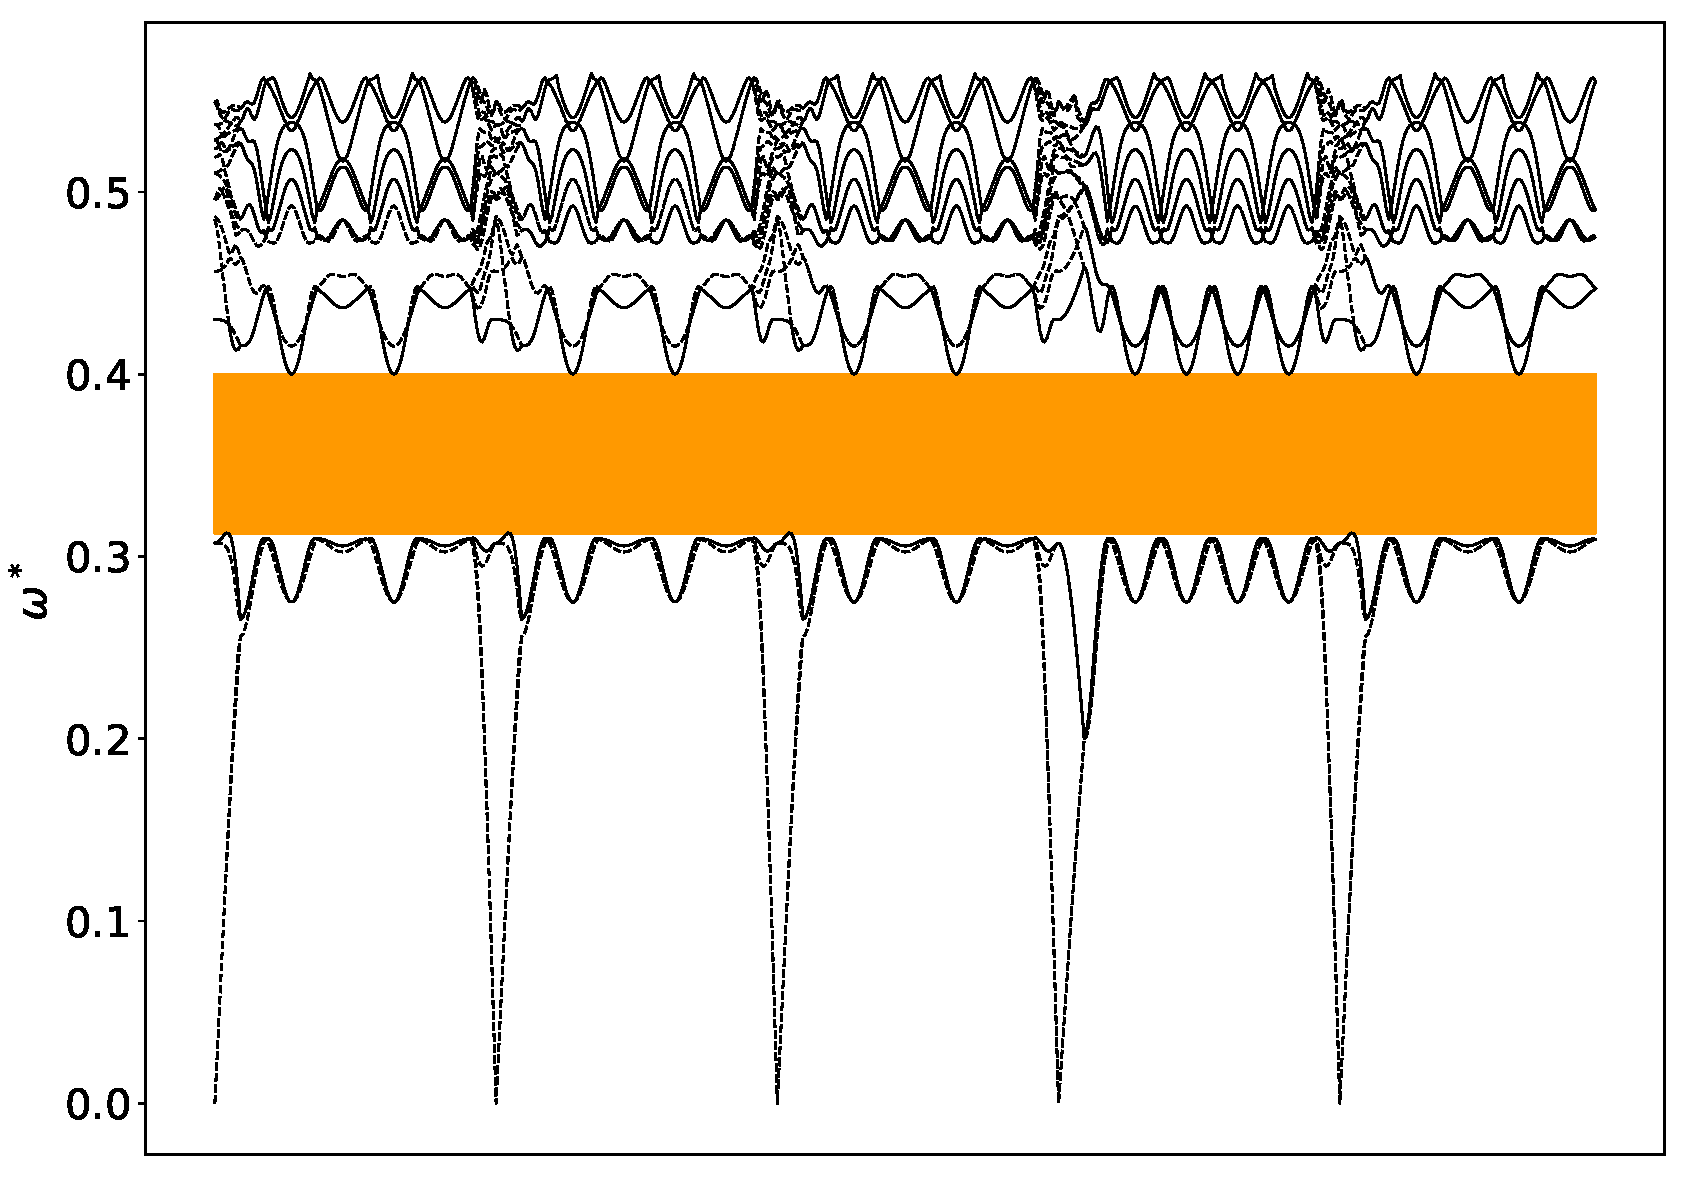
\includegraphics[width=0.9\linewidth,height=2.0in,keepaspectratio]{/Users/rosecers/work_folders/structures_for_photonics/reference/ref_inp/workspace/3ffeff60e1ef4fe0842f6f61826d67b2/./final_images/band_diagram_b=4.pdf}
\\Band Structure across 1st BZ
\end{minipage}\hfill
\begin{minipage}{0.48\textwidth}\centering
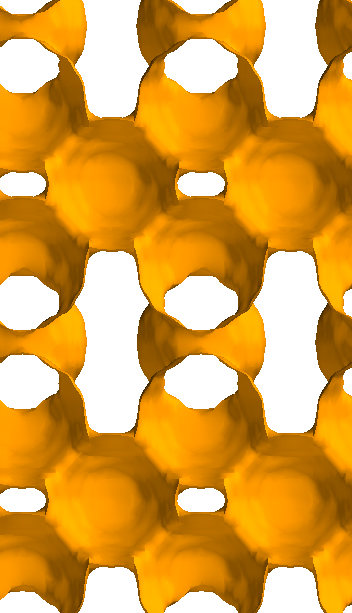
\includegraphics[width=0.9\linewidth,height=2.0in,keepaspectratio]{/Users/rosecers/work_folders/structures_for_photonics/reference/ref_inp/workspace/3ffeff60e1ef4fe0842f6f61826d67b2/final_images/tP4-PdO@gap_4-5.png}
\\View along $a_1$ 
\end{minipage}\hfill\caption{Band Structure and Isosurface of \textit{tP}4-PdO (Direct) at radius = 0.37, filling fraction = 0.621, where the largest gap between bands 4 and 5 occurs with gap size 0.18\%.}

\end{figure}
\vspace{-0.25in}


\begin{figure}[H]
\begin{minipage}{0.5\textwidth}\centering
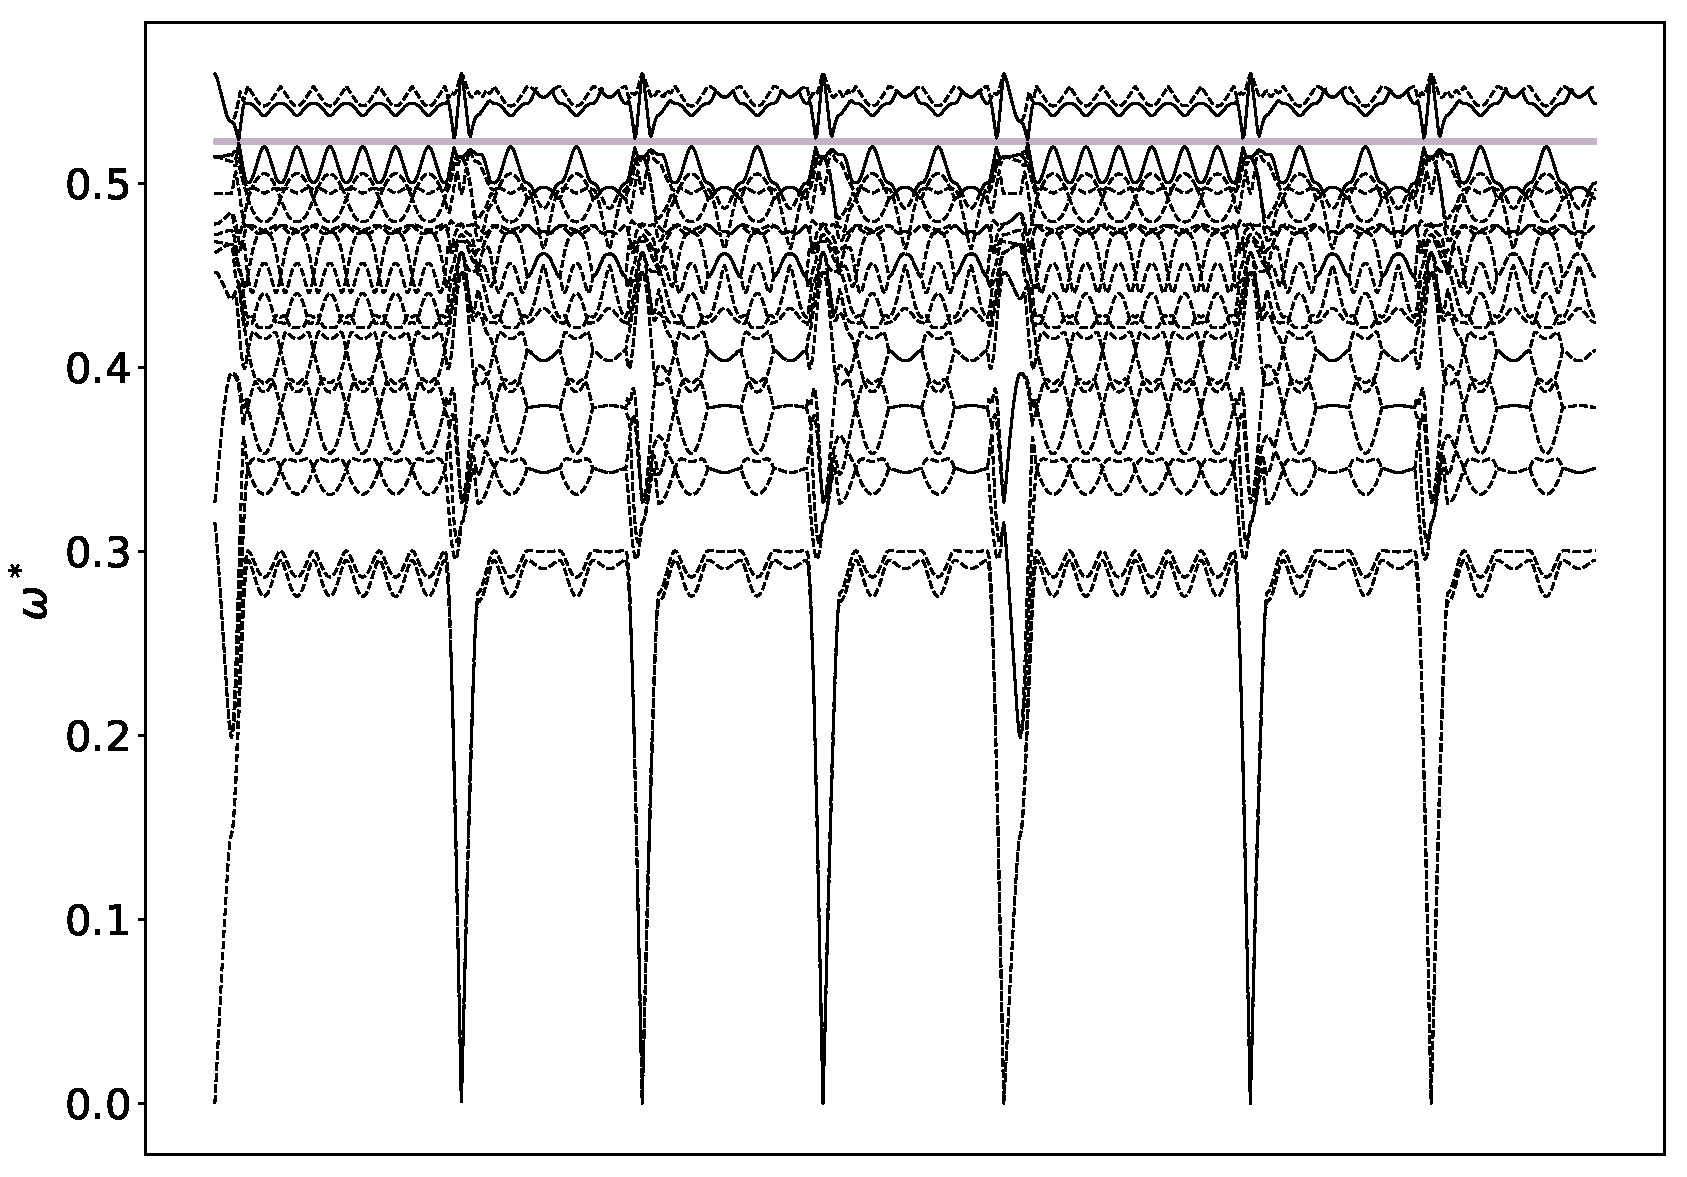
\includegraphics[width=0.9\linewidth,height=2.0in,keepaspectratio]{/Users/rosecers/work_folders/structures_for_photonics/reference/ref_inp/workspace/3ffeff60e1ef4fe0842f6f61826d67b2/./final_images/band_diagram_b=18.pdf}
\\Band Structure across 1st BZ
\end{minipage}\hfill
\begin{minipage}{0.48\textwidth}\centering
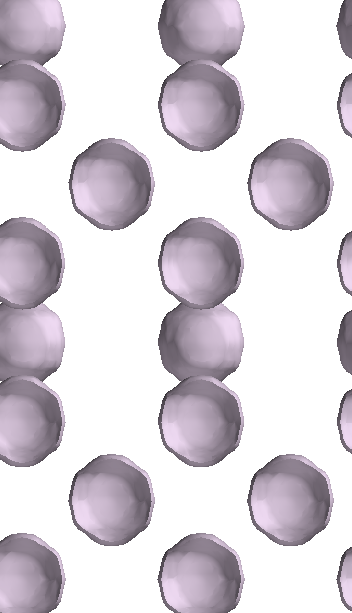
\includegraphics[width=0.9\linewidth,height=2.0in,keepaspectratio]{/Users/rosecers/work_folders/structures_for_photonics/reference/ref_inp/workspace/3ffeff60e1ef4fe0842f6f61826d67b2/final_images/tP4-PdO@gap_18-19.png}
\\View along $a_1$ 
\end{minipage}\hfill\caption{Band Structure and Isosurface of \textit{tP}4-PdO (Direct) at radius = 0.25, filling fraction = 0.257, where the largest gap between bands 18 and 19 occurs with gap size 1.28\%.}

\end{figure}
\vspace{-0.25in}

